\documentclass[11pt,a4paper,]{article}
\usepackage{lmodern}

\usepackage{amssymb,amsmath}
\usepackage{ifxetex,ifluatex}
\usepackage{fixltx2e} % provides \textsubscript
\ifnum 0\ifxetex 1\fi\ifluatex 1\fi=0 % if pdftex
  \usepackage[T1]{fontenc}
  \usepackage[utf8]{inputenc}
\else % if luatex or xelatex
  \usepackage{unicode-math}
  \defaultfontfeatures{Ligatures=TeX,Scale=MatchLowercase}
\fi
% use upquote if available, for straight quotes in verbatim environments
\IfFileExists{upquote.sty}{\usepackage{upquote}}{}
% use microtype if available
\IfFileExists{microtype.sty}{%
\usepackage[]{microtype}
\UseMicrotypeSet[protrusion]{basicmath} % disable protrusion for tt fonts
}{}
\PassOptionsToPackage{hyphens}{url} % url is loaded by hyperref
\usepackage[unicode=true]{hyperref}
\hypersetup{
            pdftitle={What does data tell us about the education situations around the world?},
            pdfborder={0 0 0},
            breaklinks=true}
\urlstyle{same}  % don't use monospace font for urls
\usepackage{geometry}
\geometry{a4paper, centering, text={16cm,24cm}}
\usepackage[style=authoryear-comp,]{biblatex}
\addbibresource{references.bib}
\usepackage{longtable,booktabs}
% Fix footnotes in tables (requires footnote package)
\IfFileExists{footnote.sty}{\usepackage{footnote}\makesavenoteenv{long table}}{}
\IfFileExists{parskip.sty}{%
\usepackage{parskip}
}{% else
\setlength{\parindent}{0pt}
\setlength{\parskip}{6pt plus 2pt minus 1pt}
}
\setlength{\emergencystretch}{3em}  % prevent overfull lines
\providecommand{\tightlist}{%
  \setlength{\itemsep}{0pt}\setlength{\parskip}{0pt}}
\setcounter{secnumdepth}{5}

% set default figure placement to htbp
\makeatletter
\def\fps@figure{htbp}
\makeatother


\title{What does data tell us about the education situations around the world?}

%% MONASH STUFF

%% CAPTIONS
\RequirePackage{caption}
\DeclareCaptionStyle{italic}[justification=centering]
 {labelfont={bf},textfont={it},labelsep=colon}
\captionsetup[figure]{style=italic,format=hang,singlelinecheck=true}
\captionsetup[table]{style=italic,format=hang,singlelinecheck=true}


%% FONT
\RequirePackage{bera}
\RequirePackage[charter,expert,sfscaled]{mathdesign}
\RequirePackage{fontawesome}

%% HEADERS AND FOOTERS
\RequirePackage{fancyhdr}
\pagestyle{fancy}
\rfoot{\Large\sffamily\raisebox{-0.1cm}{\textbf{\thepage}}}
\makeatletter
\lhead{\textsf{\expandafter{\@title}}}
\makeatother
\rhead{}
\cfoot{}
\setlength{\headheight}{15pt}
\renewcommand{\headrulewidth}{0.4pt}
\renewcommand{\footrulewidth}{0.4pt}
\fancypagestyle{plain}{%
\fancyhf{} % clear all header and footer fields
\fancyfoot[C]{\sffamily\thepage} % except the center
\renewcommand{\headrulewidth}{0pt}
\renewcommand{\footrulewidth}{0pt}}

%% MATHS
\RequirePackage{bm,amsmath}
\allowdisplaybreaks

%% GRAPHICS
\RequirePackage{graphicx}
\setcounter{topnumber}{2}
\setcounter{bottomnumber}{2}
\setcounter{totalnumber}{4}
\renewcommand{\topfraction}{0.85}
\renewcommand{\bottomfraction}{0.85}
\renewcommand{\textfraction}{0.15}
\renewcommand{\floatpagefraction}{0.8}


%\RequirePackage[section]{placeins}

%% SECTION TITLES


%% SECTION TITLES (NEW: Changing sections and subsections color)
\RequirePackage[compact,sf,bf]{titlesec}
\titleformat*{\section}{\Large\sf\bfseries\color[rgb]{0.8, 0.7, 0.1 }}
\titleformat*{\subsection}{\large\sf\bfseries\color[rgb]{0.8, 0.7, 0.1 }}
\titleformat*{\subsubsection}{\sf\bfseries\color[rgb]{0.8, 0.7, 0.1 }}
\titlespacing{\section}{0pt}{2ex}{.5ex}
\titlespacing{\subsection}{0pt}{1.5ex}{0ex}
\titlespacing{\subsubsection}{0pt}{.5ex}{0ex}


%% TITLE PAGE
\def\Date{\number\day}
\def\Month{\ifcase\month\or
 January\or February\or March\or April\or May\or June\or
 July\or August\or September\or October\or November\or December\fi}
\def\Year{\number\year}

%% LINE AND PAGE BREAKING
\sloppy
\clubpenalty = 10000
\widowpenalty = 10000
\brokenpenalty = 10000
\RequirePackage{microtype}

%% PARAGRAPH BREAKS
\setlength{\parskip}{1.4ex}
\setlength{\parindent}{0em}

%% HYPERLINKS
\RequirePackage{xcolor} % Needed for links
\definecolor{darkblue}{rgb}{0,0,.6}
\RequirePackage{url}

\makeatletter
\@ifpackageloaded{hyperref}{}{\RequirePackage{hyperref}}
\makeatother
\hypersetup{
     citecolor=0 0 0,
     breaklinks=true,
     bookmarksopen=true,
     bookmarksnumbered=true,
     linkcolor=darkblue,
     urlcolor=blue,
     citecolor=darkblue,
     colorlinks=true}

\usepackage[showonlyrefs]{mathtools}
\usepackage[no-weekday]{eukdate}

%% BIBLIOGRAPHY

\makeatletter
\@ifpackageloaded{biblatex}{}{\usepackage[style=authoryear-comp, backend=biber, natbib=true]{biblatex}}
\makeatother
\ExecuteBibliographyOptions{bibencoding=utf8,minnames=1,maxnames=3, maxbibnames=99,dashed=false,terseinits=true,giveninits=true,uniquename=false,uniquelist=false,doi=false, isbn=false,url=true,sortcites=false}

\DeclareFieldFormat{url}{\texttt{\url{#1}}}
\DeclareFieldFormat[article]{pages}{#1}
\DeclareFieldFormat[inproceedings]{pages}{\lowercase{pp.}#1}
\DeclareFieldFormat[incollection]{pages}{\lowercase{pp.}#1}
\DeclareFieldFormat[article]{volume}{\mkbibbold{#1}}
\DeclareFieldFormat[article]{number}{\mkbibparens{#1}}
\DeclareFieldFormat[article]{title}{\MakeCapital{#1}}
\DeclareFieldFormat[article]{url}{}
%\DeclareFieldFormat[book]{url}{}
%\DeclareFieldFormat[inbook]{url}{}
%\DeclareFieldFormat[incollection]{url}{}
%\DeclareFieldFormat[inproceedings]{url}{}
\DeclareFieldFormat[inproceedings]{title}{#1}
\DeclareFieldFormat{shorthandwidth}{#1}
%\DeclareFieldFormat{extrayear}{}
% No dot before number of articles
\usepackage{xpatch}
\xpatchbibmacro{volume+number+eid}{\setunit*{\adddot}}{}{}{}
% Remove In: for an article.
\renewbibmacro{in:}{%
  \ifentrytype{article}{}{%
  \printtext{\bibstring{in}\intitlepunct}}}

\AtEveryBibitem{\clearfield{month}}
\AtEveryCitekey{\clearfield{month}}

\makeatletter
\DeclareDelimFormat[cbx@textcite]{nameyeardelim}{\addspace}
\makeatother

\author{\sf\Large\textbf{ Mengyuan YANG}\\ {\sf\large Master of Business Analytics\\[0.5cm]} \sf\Large\textbf{ Zoljargal BATSAIKHAN}\\ {\sf\large Master of Business Analytics\\[0.5cm]} \sf\Large\textbf{ Xinrui WANG}\\ {\sf\large Master of Business Analytics\\[0.5cm]} \sf\Large\textbf{ Xueqi GOH}\\ {\sf\large Master of Business Analytics\\[0.5cm]}}

\date{\sf\Date~\Month~\Year}
\makeatletter
\lfoot{\sf YANG, BATSAIKHAN, WANG, GOH: \@date}
\makeatother


%%%% PAGE STYLE FOR FRONT PAGE OF REPORTS

\makeatletter
\def\organization#1{\gdef\@organization{#1}}
\def\telephone#1{\gdef\@telephone{#1}}
\def\email#1{\gdef\@email{#1}}
\makeatother
  \organization{Monash University}

  \def\name{Our consultancy \newline Mengyuan YANG \&\newline Zoljargal BATSAIKHAN \&\newline Xinrui WANG \&\newline Xueqi GOH}

  \telephone{(04) 0536 7622}

  \email{myan0065@student.monash.edu}                 %NEW: New email addresss

\def\webaddress{\url{https://github.com/xwan0274/assignment4-team-tidyverse.git}} %NEW: URl
\def\abn{NA}                                    % NEW: ABN
\def\logo{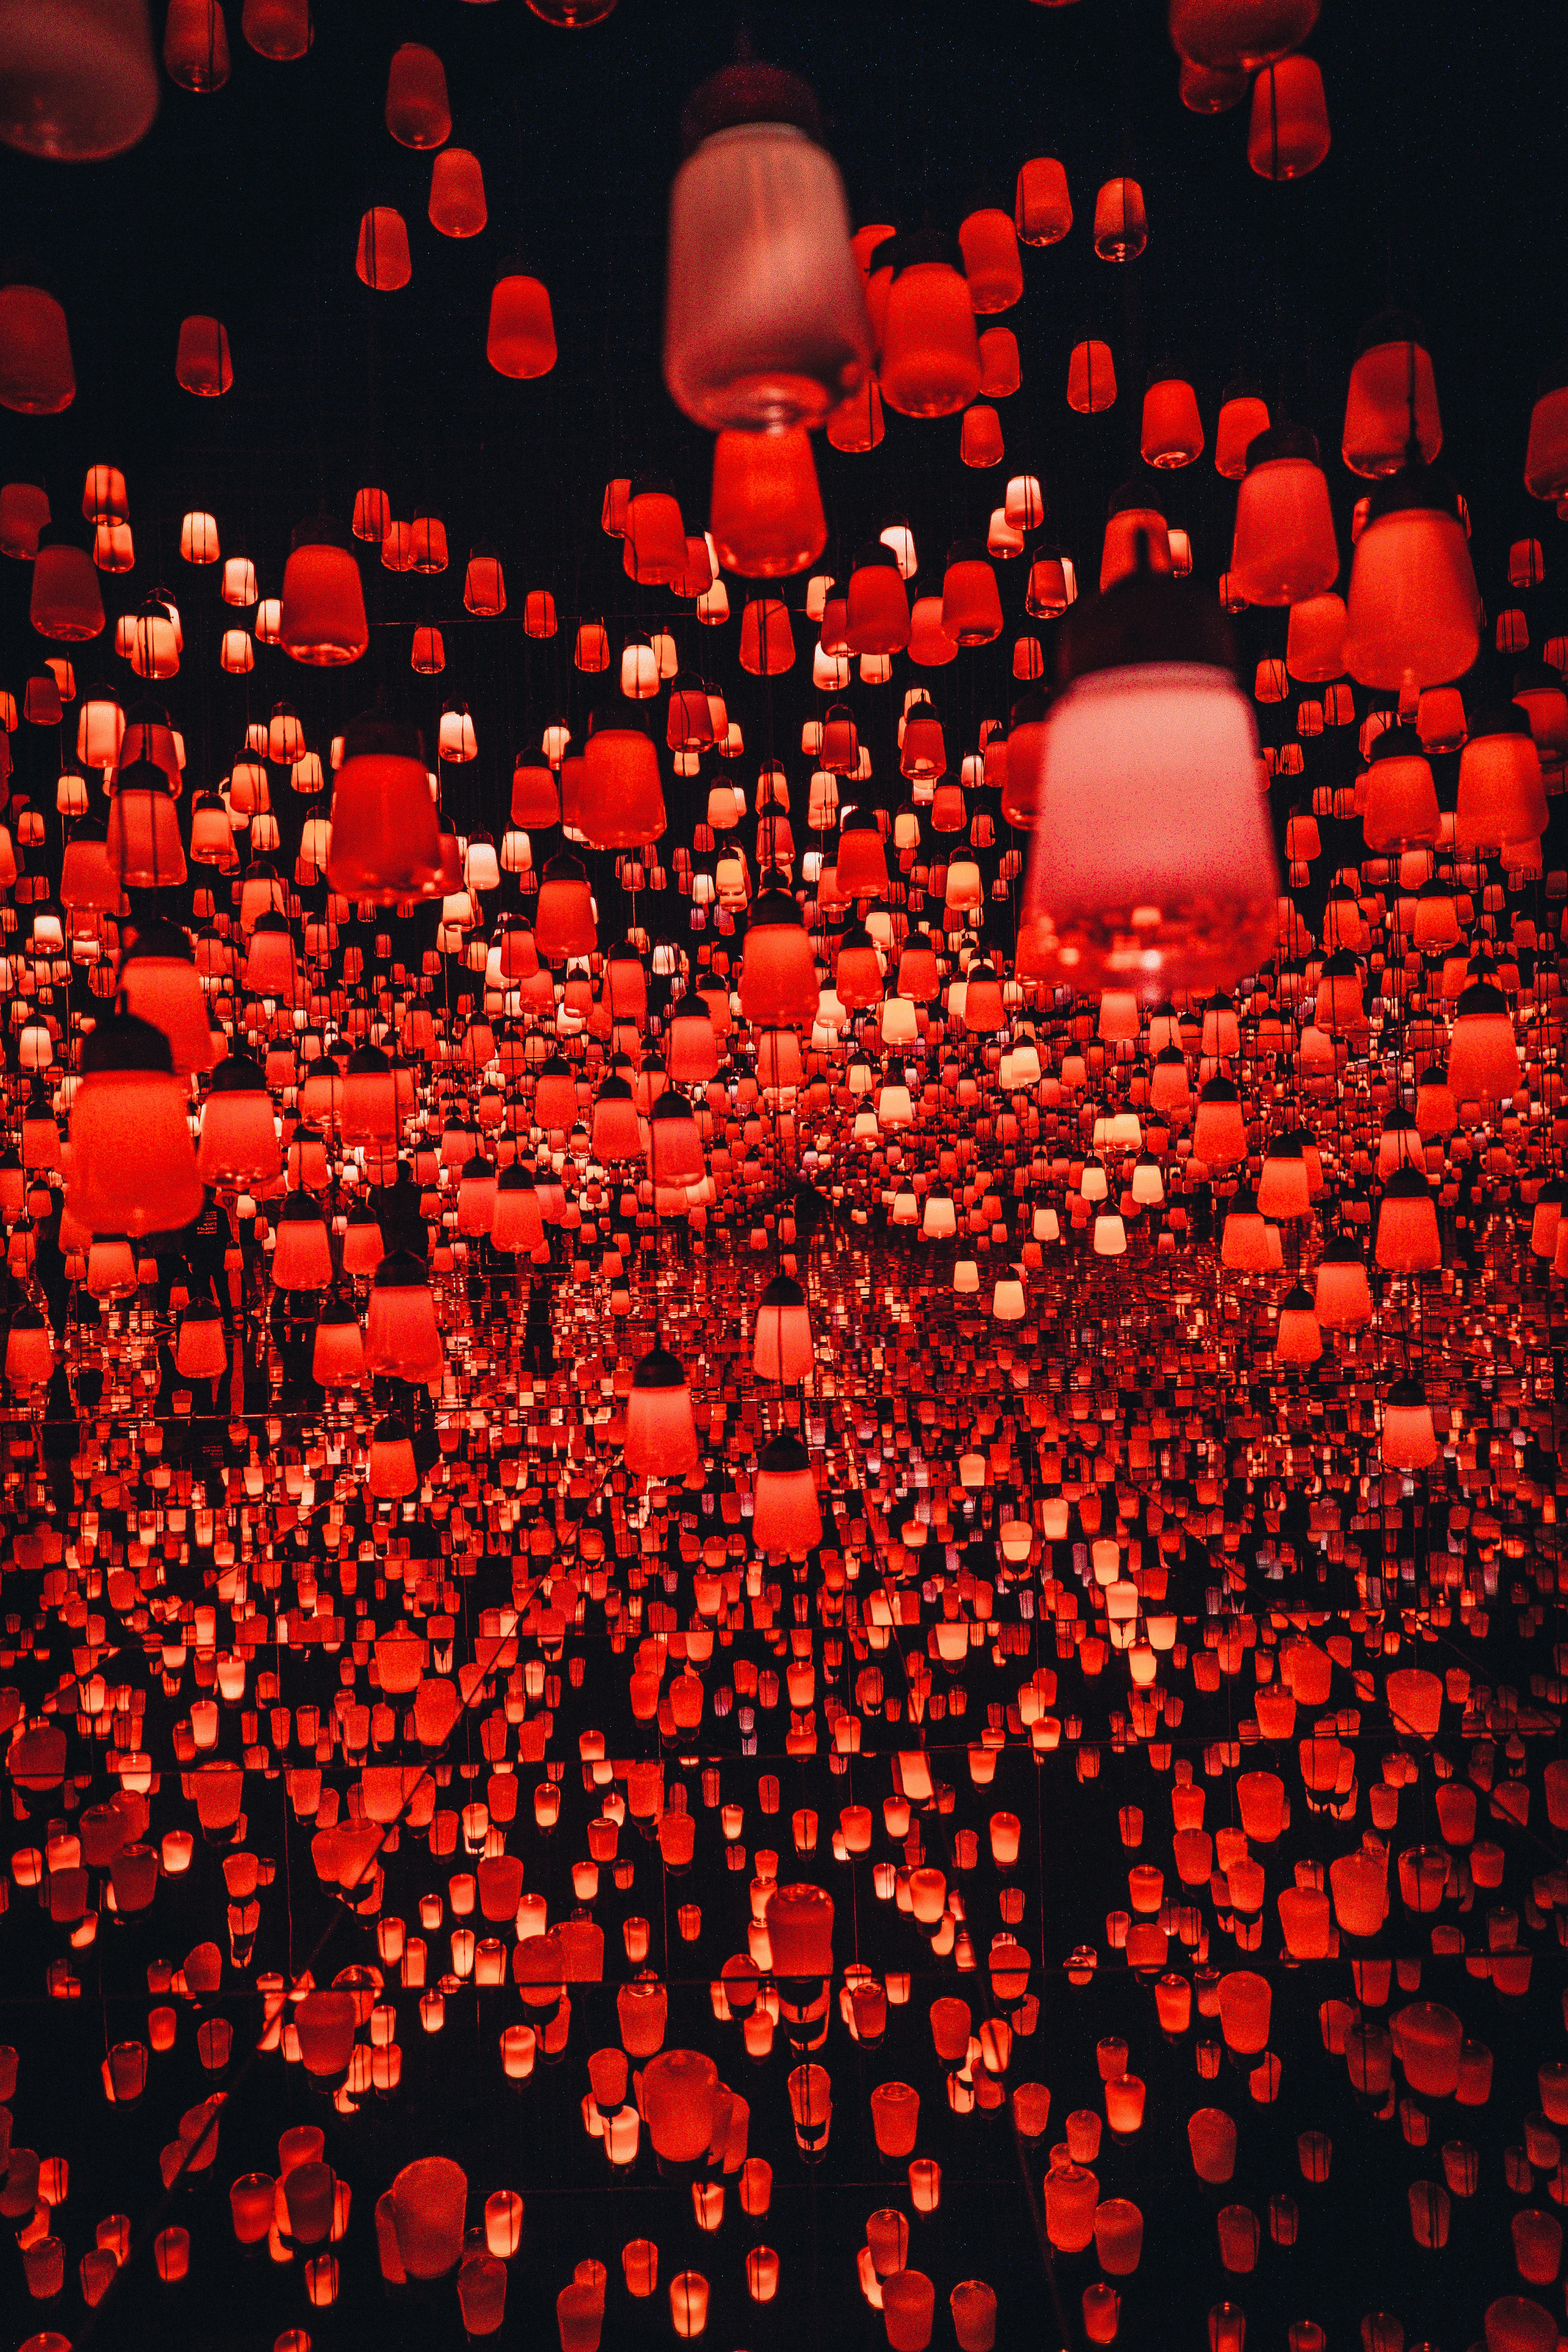
\includegraphics[width=6cm]{Figures/logo}}  %NEW: Changing logo
\def\extraspace{\vspace*{1.6cm}}
\makeatletter
\def\contactdetails{\faicon{phone} & \@telephone \\
                    \faicon{envelope} & \@email}
\makeatother

%%%% FRONT PAGE OF REPORTS

\def\reporttype{Report for}

\long\def\front#1#2#3{
\newpage
\begin{singlespacing}
\thispagestyle{empty}
\vspace*{-1.4cm}
\hspace*{-1.4cm}
\hbox to 16cm{
  \hbox to 6.5cm{\vbox to 14cm{\vbox to 25cm{
    \logo
    \vfill
    \parbox{6.3cm}{\raggedright
      \sf\color[rgb]{0.8, 0.7, 0.1 }    % NEW color 
      {\large\textbf{\name}}\par
      \vspace{.7cm}
      \tabcolsep=0.12cm\sf\small
      \begin{tabular}{@{}ll@{}}\contactdetails
      \end{tabular}
      \vspace*{0.3cm}\par
      ABN: \abn\par
    }
  }\vss}\hss}
  \hspace*{0.2cm}
  \hbox to 1cm{\vbox to 14cm{\rule{4pt}{26.8cm}\vss}\hss\hfill}  %NEW: Thicker line
  \hbox to 10cm{\vbox to 14cm{\vbox to 25cm{   
      \vspace*{3cm}\sf\raggedright
      \parbox{11cm}{\sf\raggedright\baselineskip=1.2cm
         \fontsize{24.88}{30}\color[rgb]{0, 0.29, 0.55}\sf\textbf{#1}}   % NEW: title color blue
      \par
      \vfill
      \large
      \vbox{\parskip=0.8cm #2}\par
      \vspace*{2cm}\par
      \reporttype\\[0.3cm]
      \hbox{#3}%\\[2cm]\
      \vspace*{1cm}
      {\large\sf\textbf{\Date~\Month~\Year}}
   }\vss}
  }}
\end{singlespacing}
\newpage
}

\makeatletter
\def\titlepage{\front{\expandafter{\@title}}{\@author}{\@organization}}
\makeatother

\usepackage{setspace}
\setstretch{1.5}

%% Any special functions or other packages can be loaded here.
\usepackage{float}
\usepackage{booktabs}
\usepackage{longtable}
\usepackage{array}
\usepackage{multirow}
\usepackage{wrapfig}
\usepackage{colortbl}
\usepackage{pdflscape}
\usepackage{tabu}
\usepackage{threeparttable}
\usepackage{threeparttablex}
\usepackage[normalem]{ulem}
\usepackage{makecell}
\usepackage{xcolor}


\begin{document}
\titlepage

{
\setcounter{tocdepth}{2}
\tableofcontents
}
\section*{Introduction}

\section*{Literacy Rate}

This section is to compare the literacy rate for adult and youth globally, regionally and in different age groups.

\begin{figure}[H]
\includegraphics[width=0.9\linewidth,]{report_files/figure-latex/world-my-1} \caption{Global Literacy Rate for Adult and Youth between 2000-2019}\label{fig:world-my}
\end{figure}

Figure \ref{fig:world-my} shows that although the literacy rate for adult aged 15 and above is lower that the literacy rate for youth aged 15-24 in each year, both rates are showing a slow and steady increase over the years. The improvements in the expansion of basic education and the reduction of education inequalities have contributed to an increase in the global literacy rate, over the last 65 years it increased by 4\% every 5 years (\textcite{owidliteracy}).

\begin{figure}[H]
\includegraphics[width=0.9\linewidth,]{report_files/figure-latex/regions-my-1} \caption{Global Literacy Rate for Adult and Youth between 2000-2019}\label{fig:regions-my}
\end{figure}

As the figure \ref{fig:regions-my} shown above, there was a significant increase in the literacy rate for adult aged 15 and above in Middle East \& North Africa, South Asia and Sub-Saharan Africa. South Asia and Sub-Saharan Africa also had improved the literacy rate tremendously in the youth age group over the years. Both East Asia \& Pacific and Latin America \& Caribbean had an 5\% increase in literacy rate in the adult group where as the literacy rate increase approximately 4\% in the youth group in Latin America \& Caribbean and a small increase in the youth group in East Asia \& Pacific. Regions like Central Europe and the Baltics and Europe \& Central Asia had maintained a high literacy rate in both age groups over the years. Developed countries have better education facilities and system than developing countries, they tend to have higher literacy rate over the years.

\begin{figure}[H]
\includegraphics[width=0.9\linewidth,]{report_files/figure-latex/income-my-1} \caption{Literacy Rate for Adult and Youth in Differenet Income Groups}\label{fig:income-my}
\end{figure}

Figure \ref{fig:income-my} demonstrates that both adult and youth groups that have higher income tend to have higher literacy rate and all the income groups are showing an increasing trend in the literacy rate except for the upper middle income group had maintained a very high literacy rate over the years. It's pretty obvious that people have higher income are able to afford better education compare to those people with lower income.

\section*{Education expenditure trend over the world}

In this section we will discuss education expenditure across different countries in time period of 2000 to 2019. The indicator we have chosen to analyze in this section is:

\begin{itemize}
\tightlist
\item
  Government expenditure on education, total (\% of GDP).
\end{itemize}

General government expenditure on education (current, capital, and transfers) is expressed as a percentage of Gross Domestic Product (GDP). It includes expenditure funded by transfers from international sources to government.

\textbackslash begin\{figure\}{[}H{]}
\includegraphics{report_files/figure-latex/plot1zb-1} \textbackslash caption\{Average government expenditure on education (\% of GDP), 2000-2019\}\label{fig:plot1zb}
\textbackslash end\{figure\}

Figure \ref{fig:plot1zb}, provides an overview of spending on education by country. To produce the figure, we calculated average spending over the time period for each country. The average government spending on education across countries ranged between 1.2\% - 11.5\% of their GDP.

\textbackslash begin\{figure\}{[}H{]}
\includegraphics{report_files/figure-latex/plot2-zb-1} \textbackslash caption\{Government expenditure on education (\% of GDP), by income group\}\label{fig:plot2-zb}
\textbackslash end\{figure\}

Then we looked at the government expenditure on education by income group over time in Figure \ref{fig:plot2-zb}. What evident on the graph is that the low income countries have devoted much lesser proportion of their GDP but also we can see that spending has increased on average for those countries. On the other hand, high income countries spending more share of their GDP roughly between 4.5\% to 5\%. However the data had many missing values, a broad upward trend can be observed from the Figure \ref{fig:plot2-zb}.

\textbackslash begin\{figure\}{[}H{]}
\includegraphics{report_files/figure-latex/plot3-zb-1} \textbackslash caption\{Government expenditure on education (\% of GDP), by region\}\label{fig:plot3-zb}
\textbackslash end\{figure\}

In Figure \ref{fig:plot3-zb}, we visualized the education spending by geographical regions. During the time period, South Asia and Sub-Saharan Africa had the lowest spending ranging between 3-4\% but again, the plot shows upward trend for those regions. For the other regions, it seems that it has been relatively stable over time.

\begin{table}[H]

\caption{\label{tab:plot4-zb}Total government expenditure on educationby income group in 2000 and 2015}
\centering
\begin{tabular}[t]{c|c|c|c}
\hline
Income groups & 2000 & 2015 & Percentage change\\
\hline
High income & 4.46 & 4.93 & 10.35\\
\hline
Low income & 3.33 & 3.64 & 9.46\\
\hline
Lower middle income & 4.41 & 5.05 & 14.61\\
\hline
Upper middle income & 4.46 & 4.47 & 0.02\\
\hline
\end{tabular}
\end{table}

As shown in Table \ref{tab:plot4-zb}, the increase in education spending is evident for the majority of countries. But it remained at the same level for the upper middle income countries.

Overall, it can be concluded that the total amount of global resources spent on education is increasing over the world. But according to the article \cite{trabelsi2018public}, it is suggested that if the governance is weak more public spending on education leads to lower growth. However, the improvement of the quality of institutions enhances the economic performance.

\section*{Percentage of children out of primary school}

This section discusses the percentage of primary-school-age children who are not enrolled in primary or secondary school across regions between 2000 to 2019, including the changes of overall percentage and the difference in percentage between gender over these two decades.

Figure \ref{fig:plot1xw} shows that among all of the seven regions, Sub-Saharan Africa has the highest percentage of primary-school-age children out of school, followed by South Asia and Middle East \& North Africa. However, all of these three countries witnessed a decrease in the percentage, especially in Sub-Saharan Africa, the figure dropped from nearly 40\% in 2000 to lower than 20\% in 2019. As suggested by \textcite{bennell2002hitting}, high levels of sustained enrollment growth could be observed in Sub-Sahara Africa between 2000 and 2015. The percentage in South Asia and Middle East \& North Africa also decreased to below 10\% in 2019 while the figure for rest regions remained relatively steady between 0-5\%.

\begin{figure}[H]
\includegraphics{report_files/figure-latex/plot1xw-1} \caption{Percentage of children out of school in primary school age}\label{fig:plot1xw}
\end{figure}

To have a deeper understanding, Figure \ref{fig:plot1xw} explores the difference of percentage of primary-school-age out of school in gender across regions. Again, in Middle East \& North Africa, South Asia and Sub-Saharan Africa, where the total percentage is significantly higher, it is obvious that more females in primary school age are out of school compare with males.

\begin{figure}[H]
\includegraphics{report_files/figure-latex/plot2xw-1} \caption{Percentage of children out of school in primary school age by gender}\label{fig:plot2xw}
\end{figure}

According to Table \ref{tab:tb1xw}, in South Asia, the difference in percentage between male and female was the highest in 2000, the percentage of female children out of primary school is 13.05\% higher than male. However, the difference decreased along with the total percentage, by the year of 2019, the difference in percentage has dropped to 1.26\%.

Same changes can be observed in Middle East \& North Africa, the difference in percentage also decreased from 7.33\% to 1.94\% between 2000 and 2019. Whereas in Sub-Saharan Africa, even though the total percentage drooped over the years, the difference in percentage between male and female school aged children did not decrease as much as in South Asia and Middle East \& North Africa. In 2019, the percentage of female children out of primary school is still 4.29\% higher compare with male.

\begin{table}[H]

\caption{\label{tab:tb1xw}Difference in percentage of primary-school-age children out of school between males and females}
\centering
\begin{tabular}[t]{c|c|c}
\hline
Region & Difference in percentage - 2000 & Difference in percentage - 2019\\
\hline
South Asia & 13.05 & 1.26\\
\hline
Middle East \& North Africa & 7.33 & 1.94\\
\hline
Sub-Saharan Africa & 7.16 & 4.29\\
\hline
Europe \& Central Asia & 1.09 & -0.14\\
\hline
Latin America \& Caribbean & 0.91 & -0.56\\
\hline
East Asia \& Pacific & 0.72 & 0.84\\
\hline
North America & 0.23 & 0.11\\
\hline
\end{tabular}
\end{table}

Another interesting finding is that in Europe \& Central Asia and Latin America \& Caribbean, the difference in percentage is -0.14\% and -0.56\% respectively in 2019, which indicates that in 2019, the percentage of primary-school-age male who are not enrolled in primary or secondary school is actually slightly higher than female, although the difference is very close to zero (Table \ref{tab:tb1xw}).

\section*{Xueqi}

This section discuss the pupil-teacher ratio from 2000-2019

\includegraphics{report_files/figure-latex/figure1-1}

Figure \ref{fig:figure1} Pupil-teacher ratio seems similar across 2000-2018. However, in 2019, there's a significant decrease in pupil-teacher ratio especially in tertiary level and primary level. Next, there's an increase pupil-teacher ratio in upper secondary level, secondary level and lower secondary level.

\begin{table}

\caption{\label{tab:Table2}Regional Average Pupil-teacher ratio between 2000-2019}
\centering
\begin{tabular}[t]{l|l|r}
\hline
Indicator & Region & Average\_ratio\\
\hline
Pupil-teacher ratio, lower secondary & North America & 7.883399\\
\hline
Pupil-teacher ratio, secondary & North America & 7.979289\\
\hline
Pupil-teacher ratio, preprimary & North America & 9.078012\\
\hline
Pupil-teacher ratio, upper secondary & North America & 9.125136\\
\hline
Pupil-teacher ratio, primary & North America & 10.210233\\
\hline
Pupil-teacher ratio, lower secondary & Europe \& Central Asia & 10.472160\\
\hline
Pupil-teacher ratio, secondary & Europe \& Central Asia & 11.001635\\
\hline
Pupil-teacher ratio, upper secondary & Europe \& Central Asia & 12.030519\\
\hline
Pupil-teacher ratio, tertiary & North America & 12.085918\\
\hline
Pupil-teacher ratio, preprimary & Europe \& Central Asia & 12.700575\\
\hline
Pupil-teacher ratio, upper secondary & Middle East \& North Africa & 12.831898\\
\hline
Pupil-teacher ratio, tertiary & Latin America \& Caribbean & 13.020706\\
\hline
Pupil-teacher ratio, tertiary & Europe \& Central Asia & 14.475969\\
\hline
Pupil-teacher ratio, secondary & Middle East \& North Africa & 14.811131\\
\hline
Pupil-teacher ratio, primary & Europe \& Central Asia & 14.839421\\
\hline
Pupil-teacher ratio, upper secondary & Latin America \& Caribbean & 15.641246\\
\hline
Pupil-teacher ratio, lower secondary & Middle East \& North Africa & 15.967261\\
\hline
Pupil-teacher ratio, secondary & Latin America \& Caribbean & 16.471384\\
\hline
Pupil-teacher ratio, lower secondary & Latin America \& Caribbean & 17.696099\\
\hline
Pupil-teacher ratio, preprimary & South Asia & 17.959625\\
\hline
Pupil-teacher ratio, preprimary & Middle East \& North Africa & 17.971469\\
\hline
Pupil-teacher ratio, tertiary & East Asia \& Pacific & 18.230038\\
\hline
Pupil-teacher ratio, secondary & East Asia \& Pacific & 18.814013\\
\hline
Pupil-teacher ratio, upper secondary & East Asia \& Pacific & 19.035888\\
\hline
Pupil-teacher ratio, preprimary & Latin America \& Caribbean & 19.303227\\
\hline
Pupil-teacher ratio, primary & Middle East \& North Africa & 19.411776\\
\hline
Pupil-teacher ratio, tertiary & Middle East \& North Africa & 20.082141\\
\hline
Pupil-teacher ratio, lower secondary & East Asia \& Pacific & 20.270048\\
\hline
Pupil-teacher ratio, primary & Latin America \& Caribbean & 20.330124\\
\hline
Pupil-teacher ratio, tertiary & Sub-Saharan Africa & 20.578647\\
\hline
Pupil-teacher ratio, preprimary & East Asia \& Pacific & 20.920228\\
\hline
Pupil-teacher ratio, upper secondary & Sub-Saharan Africa & 21.345747\\
\hline
Pupil-teacher ratio, tertiary & South Asia & 22.264410\\
\hline
Pupil-teacher ratio, upper secondary & South Asia & 23.370092\\
\hline
Pupil-teacher ratio, primary & East Asia \& Pacific & 23.503276\\
\hline
Pupil-teacher ratio, secondary & Sub-Saharan Africa & 25.207200\\
\hline
Pupil-teacher ratio, lower secondary & South Asia & 26.102560\\
\hline
Pupil-teacher ratio, secondary & South Asia & 26.190960\\
\hline
Pupil-teacher ratio, preprimary & Sub-Saharan Africa & 27.359228\\
\hline
Pupil-teacher ratio, lower secondary & Sub-Saharan Africa & 31.375117\\
\hline
Pupil-teacher ratio, primary & South Asia & 31.633370\\
\hline
Pupil-teacher ratio, primary & Sub-Saharan Africa & 41.887322\\
\hline
\end{tabular}
\end{table}

\begin{table}

\caption{\label{tab:Table3}Regional Average Pupil-teacher ratio between 2000-2019}
\centering
\begin{tabular}[t]{l|l|r}
\hline
Indicator & Region & Average\_ratio\\
\hline
Pupil-teacher ratio, primary & Sub-Saharan Africa & 41.887322\\
\hline
Pupil-teacher ratio, primary & South Asia & 31.633370\\
\hline
Pupil-teacher ratio, lower secondary & Sub-Saharan Africa & 31.375117\\
\hline
Pupil-teacher ratio, preprimary & Sub-Saharan Africa & 27.359228\\
\hline
Pupil-teacher ratio, secondary & South Asia & 26.190960\\
\hline
Pupil-teacher ratio, lower secondary & South Asia & 26.102560\\
\hline
Pupil-teacher ratio, secondary & Sub-Saharan Africa & 25.207200\\
\hline
Pupil-teacher ratio, primary & East Asia \& Pacific & 23.503276\\
\hline
Pupil-teacher ratio, upper secondary & South Asia & 23.370092\\
\hline
Pupil-teacher ratio, tertiary & South Asia & 22.264410\\
\hline
Pupil-teacher ratio, upper secondary & Sub-Saharan Africa & 21.345747\\
\hline
Pupil-teacher ratio, preprimary & East Asia \& Pacific & 20.920228\\
\hline
Pupil-teacher ratio, tertiary & Sub-Saharan Africa & 20.578647\\
\hline
Pupil-teacher ratio, primary & Latin America \& Caribbean & 20.330124\\
\hline
Pupil-teacher ratio, lower secondary & East Asia \& Pacific & 20.270048\\
\hline
Pupil-teacher ratio, tertiary & Middle East \& North Africa & 20.082141\\
\hline
Pupil-teacher ratio, primary & Middle East \& North Africa & 19.411776\\
\hline
Pupil-teacher ratio, preprimary & Latin America \& Caribbean & 19.303227\\
\hline
Pupil-teacher ratio, upper secondary & East Asia \& Pacific & 19.035888\\
\hline
Pupil-teacher ratio, secondary & East Asia \& Pacific & 18.814013\\
\hline
Pupil-teacher ratio, tertiary & East Asia \& Pacific & 18.230038\\
\hline
Pupil-teacher ratio, preprimary & Middle East \& North Africa & 17.971469\\
\hline
Pupil-teacher ratio, preprimary & South Asia & 17.959625\\
\hline
Pupil-teacher ratio, lower secondary & Latin America \& Caribbean & 17.696099\\
\hline
Pupil-teacher ratio, secondary & Latin America \& Caribbean & 16.471384\\
\hline
Pupil-teacher ratio, lower secondary & Middle East \& North Africa & 15.967261\\
\hline
Pupil-teacher ratio, upper secondary & Latin America \& Caribbean & 15.641246\\
\hline
Pupil-teacher ratio, primary & Europe \& Central Asia & 14.839421\\
\hline
Pupil-teacher ratio, secondary & Middle East \& North Africa & 14.811131\\
\hline
Pupil-teacher ratio, tertiary & Europe \& Central Asia & 14.475969\\
\hline
Pupil-teacher ratio, tertiary & Latin America \& Caribbean & 13.020706\\
\hline
Pupil-teacher ratio, upper secondary & Middle East \& North Africa & 12.831898\\
\hline
Pupil-teacher ratio, preprimary & Europe \& Central Asia & 12.700575\\
\hline
Pupil-teacher ratio, tertiary & North America & 12.085918\\
\hline
Pupil-teacher ratio, upper secondary & Europe \& Central Asia & 12.030519\\
\hline
Pupil-teacher ratio, secondary & Europe \& Central Asia & 11.001635\\
\hline
Pupil-teacher ratio, lower secondary & Europe \& Central Asia & 10.472160\\
\hline
Pupil-teacher ratio, primary & North America & 10.210233\\
\hline
Pupil-teacher ratio, upper secondary & North America & 9.125136\\
\hline
Pupil-teacher ratio, preprimary & North America & 9.078012\\
\hline
Pupil-teacher ratio, secondary & North America & 7.979289\\
\hline
Pupil-teacher ratio, lower secondary & North America & 7.883399\\
\hline
\end{tabular}
\end{table}

Table \ref{tab:Table2} and Table \ref{tab:Table3} indicates that the highest average ratio is 41.887322 in Sub-saharan Africa's primary level between 2000-2019 holding other variable constant. Holding other variable constant, the lowest average ratio is 7.883399 in North America's lower-secondary level between 2000-2019

\includegraphics{report_files/figure-latex/figure2-1}

Figure \ref{fig:figure2} Interestingly, it seems that Sub-Saharan Africa, South Asia and Middle East \& North Africa has greater proportion in low income group comparing to other countries. Middle East \& North Africa and Sub-Saharan Africa has greater average pupil-teacher ratio in primary level. Europe\& Central Asia has similar average pupil-teacher ratio across region. East Asia \& Pacific and Latin America \& Caribbean has similar average pupil-teacher ratio. Significantly, pupil-teacher ratios are very essential to quality of education. They perhaps rank alongside professional knowledge, skill, as well as strategies, in genuinely determining educational success and performance (\textcite{ikediashi2012pupil}).

\section*{Conclusion}

\printbibliography

\end{document}
